\section{Ruta 2: Universidad de Ghana}

Ejecutamos la herramienta usando la dirección \texttt{www.ug.edu.gh}, y al igual que en el caso anterior con ráfagas de 100 paquetes y TTL máximo 30.

Realizamos un gráfico de la ruta obtenida usando una página de geolocalización por IP \cite{ip2location}, que se encuentra en la figura \ref{mapa2}.

\subsection{Análisis de la ruta obtenida}

La ruta parte de Buenos Aires, que es consistente ya que los paquetes fueron enviados desde ahí. Luego de no obtener respuesta en varios saltos, la siguiente respuesta sigue en Buenos Aires.

La ruta sigue en Estados Unidos, es posible que se utilice esta ruta a pesar de haber una más corta (según el mapa de cables subacuáticos \cite{cables}) porque al ser más utilizadas las comunicaciones entre Argentina y América del Norte (particularmente Estados Unidos) que con África, es posible que los paquetes vayan más rápido por esa ruta.

Luego hace un salto a Londres, que sería el segundo salto intercontinental. Siguiente, hace un salto a Singapur, que podría pensarse que se trata de un error de geolocalización. Sin embargo, el RTT es consistente con un envío por una ruta muy larga. De todas formas buscamos otras fuentes y vimos que la IP \texttt{195.219.195.42} podría estar ubicada en Inglaterra.

Luego los paquetes realizan varios saltos en Ghana hasta llegar a destino. 

Los saltos Buenos Aires-Ashburn, Ashburn-Londres y Singapur-Ghana son detectados correctamente. A la vez, hay muchos falsos positivos, en el caso del salto Londres-Singapur es entendible porque es un salto con un RTT muy alto, en los otros casos, pensamos que podría deberse a la aparición de RTTs con diferencia negativa con el salto anterior, que hacen que la detección de outliers sea peor.

\subsection{Análisis de las predicciones de salto intercontinental}

Calculamos las siguientes métricas de acuerdo a lo observado en la tabla \ref{tabla2}:

\begin{itemize}
	\item Porcentaje de saltos que no responden: 0\%
	\item Largo de la ruta de saltos que responden: 19 saltos 
	\item Cantidad de enlaces intercontinentales (separando América del Sur/Norte): 4
	\item Cantidad de outliers: 3
	\item Falsos positivos: 1
	\item Falsos negativos: 2
\end{itemize}

\begin{figure}[H]
\centering
\begin{tabular}{l | l | c | l | l | c | c}
Hop & RTT & Dif. de RTT & IP & Ubicación & Predicción de SI & ¿correcto?\\
\hline
1 & 0.0021 & 0.0021 & \texttt{192.168.10.1} & Buenos Aires, Argentina & false & \cmark\\
2 & 0.0060 & 0.0039 & \texttt{192.168.0.1} & Buenos Aires, Argentina & false & \cmark\\
3 & 0.0167 & 0.0107 & \texttt{10.31.0.1} & Buenos Aires, Argentina & false & \cmark\\
4 & 0.0141 & < 0 & \texttt{10.242.2.133} & Buenos Aires, Argentina & false & \cmark\\
5 & 0.0133 & < 0 & \texttt{195.22.220.33} & Buenos Aires, Argentina & false & \cmark\\
6 & 0.0147 & 0.0014 & \texttt{195.22.220.32} & Buenos Aires, Argentina & false & \cmark\\
7 & 0.1584 & 0.1437 & \texttt{195.22.199.191} & Ashburn, EEUU & true & \cmark\\
8 & 0.1714 & 0.013 & \texttt{216.6.87.202} & Ashburn, EEUU & false & \cmark\\
9 & 0.2308 & 0.0594 & \texttt{216.6.87.138} & Newark, EEUU & true & \xmark\\
10 & 0.2228 & < 0 & \texttt{216.6.57.1} & Newark, EEUU & false & \cmark\\
11 & 0.2224 & < 0 & \texttt{80.231.130.33} & Londres, Inglaterra & false & \xmark\\
12 & 0.2251 & 0.0027 & \texttt{80.231.130.130} & Londres, Inglaterra & false & \cmark\\
13 & 0.2218 & < 0 & \texttt{80.231.76.121} & Londres, Inglaterra & false & \cmark\\
14 & 0.5116 & 0.2898 & \texttt{195.219.195.42} & Singapur/Londres & true & \cmark\\
15 & 0.3219 & < 0 & \texttt{41.204.60.149} & Kumasi, Ghana & false & \xmark\\
16 & 0.3336 & 0.0117 & \texttt{41.204.60.150} & Kumasi, Ghana & false & \cmark\\
17 & 0.3298 & < 0 & \texttt{197.255.127.6} & Accra, Ghana & false & \cmark\\
18 & 0.3453 & 0.0155 & \texttt{197.255.127.35} & Accra, Ghana & false & \cmark\\
19 & 0.3393 & < 0 & \texttt{197.255.125.213} & Accra, Ghana & false & \cmark\\
\end{tabular}
\caption{Tabla de resultados para la Universidad de Ghana.}
\label{tabla2}
\end{figure}

\begin{figure}[H]
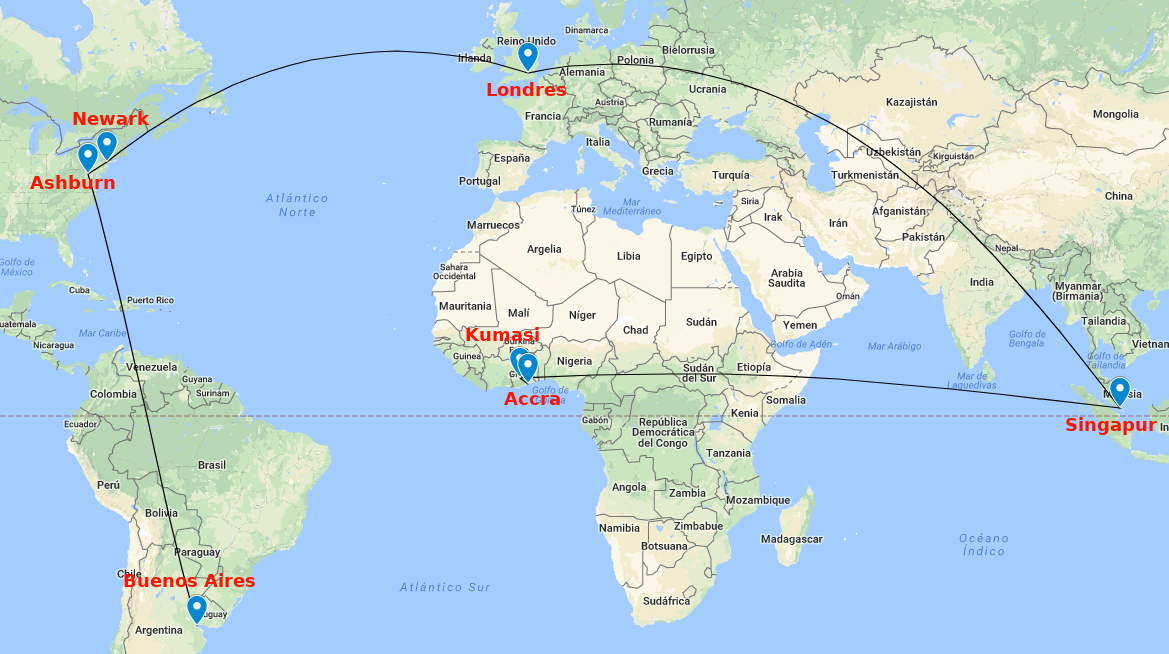
\includegraphics[width=\textwidth]{ghana.png}
\caption{Mapa de resultados para la Universidad de Ghana.}
\label{mapa2}
\end{figure}

En la figura \ref{diff1} se puede ver que la mayor diferencia se da en el salto 15, esto tiene sentido porque es el salto que va a Singapur. Aunque el siguiente salto es un salto con menor RTT, por lo que la herramienta no siempre debe estar tomando este salto. El resto de los puntos no muestran una tendencia definida (ni creciente ni decreciente).


\begin{figure}[H]
\centering
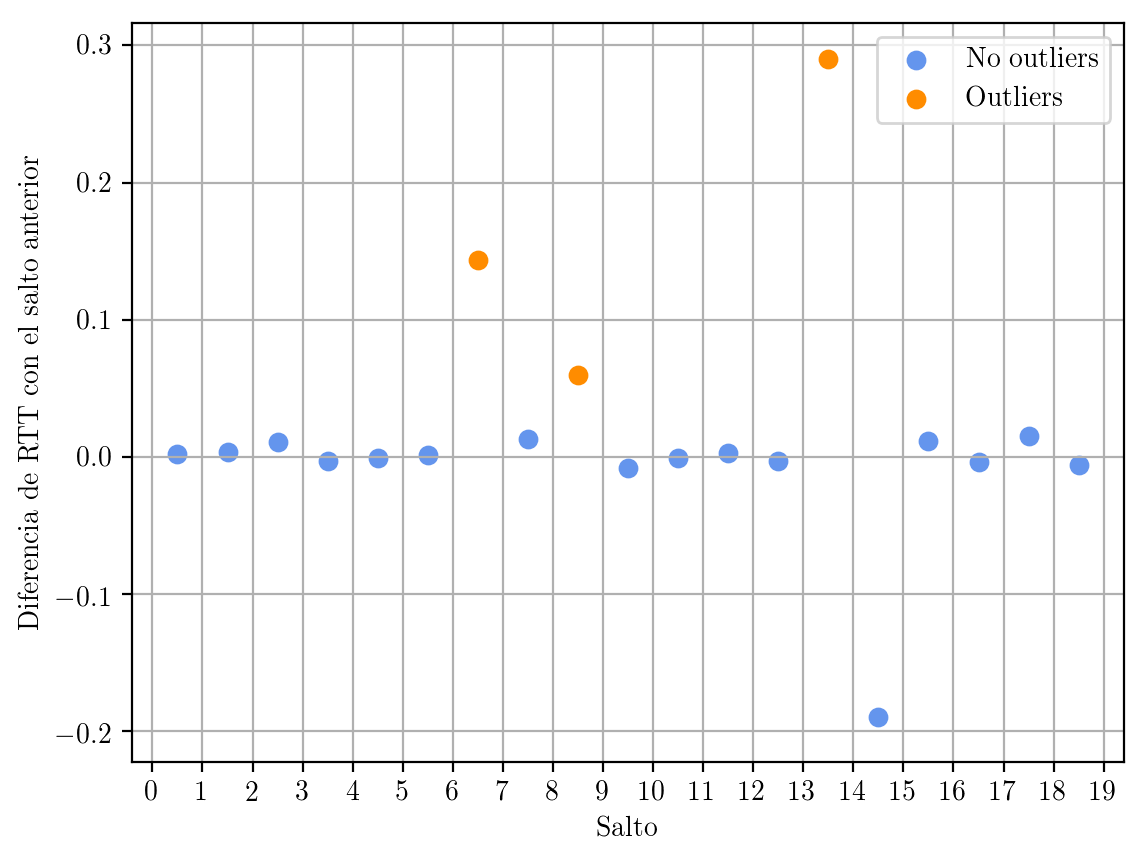
\includegraphics[width=0.6\textwidth]{ghana1.png}
\caption{Gráfico de diferencias de RTT en función de cada salto.}
\label{diff2}
\end{figure}

De la figura \ref{sdev2} vemos que también hay varios puntos están muy dispersos y por eso este experimento también devolvió muchos outliers como resultado.

\begin{figure}[H]
\centering
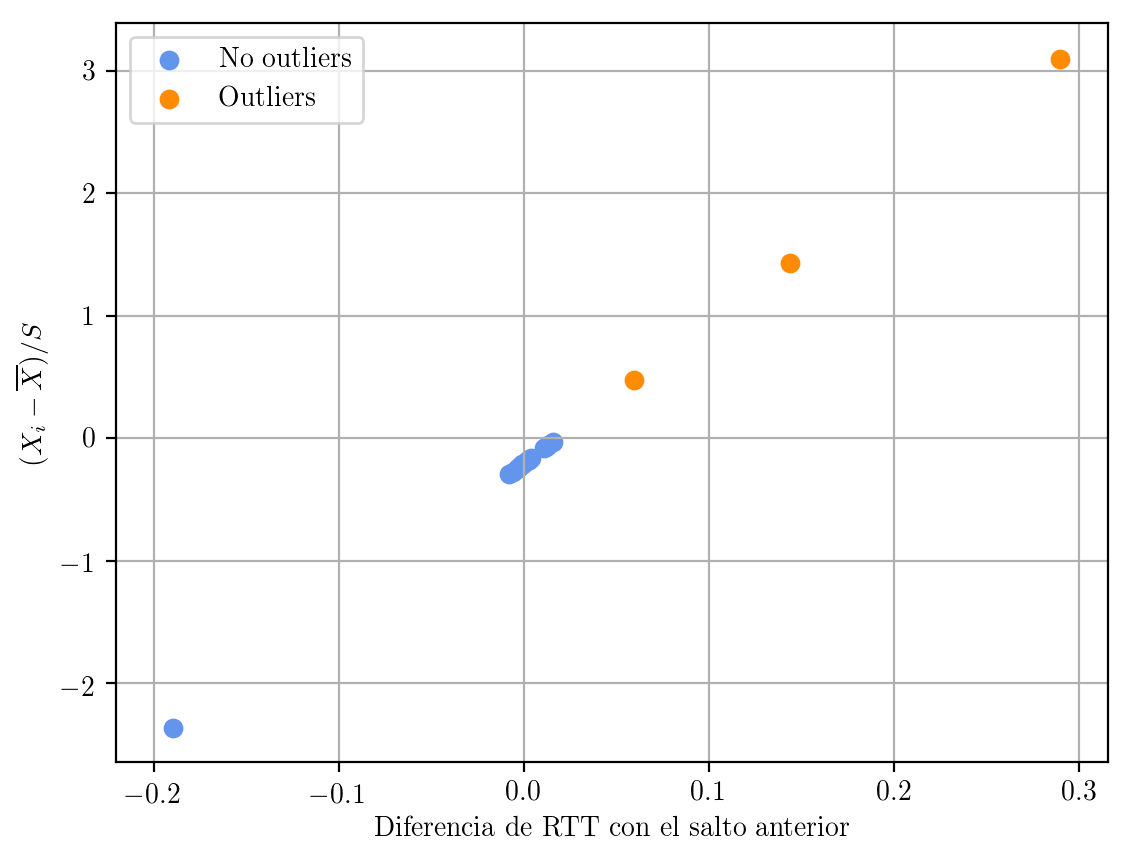
\includegraphics[width=0.6\textwidth]{ghana2.png}
\caption{Gráfico de $\frac{X_i - \bar{X}}{S}$ en función de las diferencias de RTT.}
\label{sdev2}
\end{figure}